\documentclass[a4paper,11pt,twocolumn]{article}

\usepackage{icphs2015}
\usepackage{metalogo} % Only needed for the XeLaTeX logo

\title{Effects of attention and lexical bias on perceptual learning}
\author{XXX and XXX}
\organization{XXX}
\email{XXX and XXX}
\begin{document}

\maketitle

\begin{abstract}
This paper presents the results of an experiment looking at perceptual learning when lexical bias and phonetic attention are manipulated.  All listeners exposed to an ambiguous sound halfway between an /s/ and a /ʃ/ in word contexts for /s/ adapted their /s/-/ʃ/ category boundary.  Listeners who were only exposed to the ambiguous sound in final syllable adapted their category boundary more than listeners who were exposed to the ambiguous sound at the beginnings of words, but only when they were not explicitly instructed to pay attention to the speaker's ambiguous /s/ sounds.  
\end{abstract}

\keywords{perceptual learning, lexical bias, attention}


\section{Introduction}

Perceptual learning in speech perception is a robust effect whereby listeners exposed to a novel characteristic of a speaker adapt their perceptual system to that characteristic.  For instance, if a speaker produces /s/ or /f/ in a way that sounds more like the other, and the context is clear what the intended production was, listeners will expand the intended category at the expense of the other \cite{Norris2003}.  The context that these ambiguous sounds are embedded is crucial.  If they are embedded in nonwords, no perceptual learning occurs. 

While lexical status is potentially binary, words can differ in how much they bias listeners to interpret ambiguous sounds as the category intended.  When ambiguous fricatives between /s/ and /ʃ/ are embedded earlier in a word, such as in \emph{serenade} or \emph{chandelier}, participants are more likely to treat these words as nonword than when the same ambiguous fricatives are embedded later in a word, such as \emph{establish} or \emph{embarass} \cite{Pitt2012}.  The lexical bias acting on the ambiguous fricative increases as a function of position.  However, attention can modulate this lexical bias.  When listeners were told that the speaker's /s/ and /ʃ/ were ambiguous and to listen carefully to ensure correct responses, they were less tolerant of noncanonical productions across all positions in the word \cite{Pitt2012}.  That is, participants attending to the speaker's sibilants were less likely to accept the ambiguous production as a word than participants given no particular instructions about the sibilants.

The experiment in this paper looks at perceptual learning under gradient lexical bias from modulating the position in the word of the ambiguous sibilant to be adapted to and the participants' attention to those ambiguous sibilants.  We hypothesize that perceptual learning effects will be larger for participants who were exposed the ambiguous sound embedded later in the word than participants exposed to the ambiguous sound embedded earlier in the words, and that drawing participants' attention to the ambiguous sounds lessen the perceptual learning effect.

\section{Methodology}

\subsection{Participants}

One hundred native speakers of English (mean age ??, range ??-??) participated in the experiment and were compensated with either \$10 CAD or course credit. They were recruited from the UBC student population.  Twenty additional native English speakers participated in a pretest to determine the most ambiguous sounds.  Twenty five other native speakers of English participated for course credit in a control experiment.

\subsection{Materials}

One hundred and forty English words and 100 nonwords that were phonologically legal in English were used as exposure materials.  The set of words consisted of 40 critical items, 20 control items and 60 filler words.  Half of the critical items had an /s/ in the onset of the first syllable and half had an /s/ in the onset of the final syllable.  All critical tokens formed nonwords if their /s/ was replaced with /ʃ/. Half the control items had an /ʃ/ in the onset of the first syllable and half had an /ʃ/ in the onset of the final syllable.  Each critical item and control item contained just the one sibilant, with no other /s z ʃ ʒ tʃ or dʒ/.  Filler words and nonwords did not contain any sibilants.

Four monosyllabic minimal pairs of voiceless sibilants were selected as test items for categorization (\emph{sack}-\emph{shack}, \emph{sigh}-\emph{shy}, \emph{sin}-\emph{shin}, and \emph{sock}-\emph{shock}).  Two of the pairs had a higher frequency in SUBTLEXus \cite{Brysbaert2009} for the /s/ word, and two had higher frequency for the /ʃ/ word.

All words and nonwords were recorded by a male Vancouver English speaker in quiet room.  Critical words for the exposure phase were recorded in pairs, once normally and once with the sibilant swapped forming a nonword.  The speaker was instructed to produce both forms with comparable speech rate, speech style and prosody.

For each critical item, the word and nonword versions were morphed together in an 11-step continuum (0\%-100\% of the nonword /ʃ/ recording, in steps of 10\%) using STRAIGHT \cite{Kawahara2008}.  Prior to morphing, the word and nonword versions were time aligned based on acoustic landmarks, like stop bursts, onset of F2, nasalization or frication, etc.  All control items and filler words were processed and resynthesized by STRAIGHT to ensure a consistent quality across stimulus items.  A pretest for both the exposure and categorization stimuli was performed to find the 50\% cross over point for each continuum.  For the exposure continua, the step closest to 50\% crossover was used as the exposure stimuli for that item, and for the categorization continua, three steps on either side of the cross over point were used as stimuli for categorization.

\subsection{Procedure}

Participants in the experimental conditions completed two tasks, an exposure task and a categorization task.  The exposure task was a lexical decision task, where participants heard auditory stimuli and were instructed to respond with either "word" if they thought what they heard was a word or "nonword" if they didn't think it was a word.  The buttons corresponding to "word" and "nonword" were counterbalanced across participants. Trial order was pseudorandom, with no critical or control items appearing in the first six trials, and no critical or control trials in a row, but random otherwise, following \cite{Reinisch2013}.

In the categorization task, participants heard an auditory stimulus and had to categorize it as one of two words, differing only in the onset sibilant (s vs sh).  The buttons corresponding to the words were counterbalanced across participants.  The six most ambiguous steps of the minimal pair continua were used with seven repetitions each, giving a total of 168 trials. Participants were instructed that there would two tasks in the experiment, and both tasks were explained at the beginning to remove experimenter interaction between exposure and categorization.  

Participants were assigned to one of four conditions.  Two of the conditions exposed participants to only criticall items that began with /s/, and the other two exposed them to only critical items that had an /s/ in the onset of the final syllable, giving a consistent 200 trials in all exposure phases with control and filler items shared across all participants.  Additionally participants in half the conditions received additional instructions that the speaker's "s" sounds were sometimes ambiguous, and to listen carefully to ensure correct responses in the lexical decision.

\section{Results}

\subsection{Exposure}

\subsection{Categorization}

\begin{figure*}[!ht]
\caption{Categorization as a function of step, exposure type and attention.}\label{fig:categ}
\begin{center}
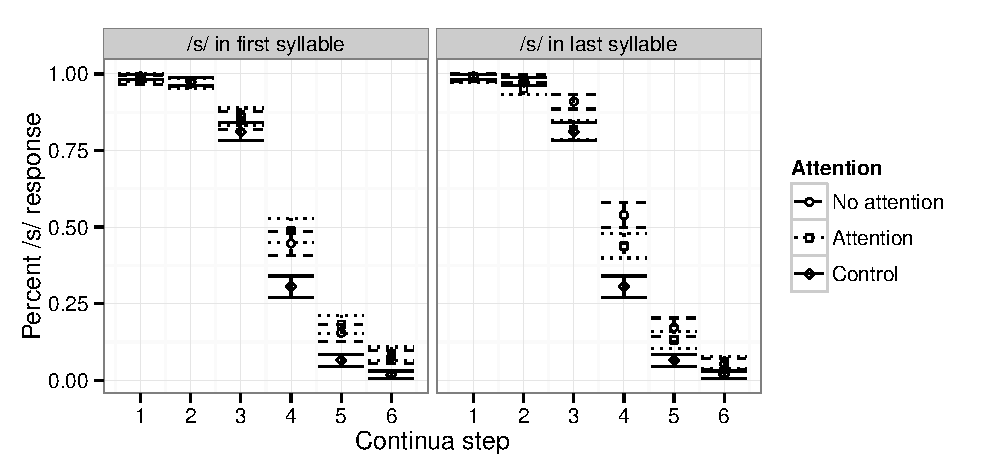
\includegraphics[width=\textwidth]{categresults}
\end{center}
\end{figure*}

Responses with reaction time less than 200 ms or greater than 2500 ms were exlcuded from analyses.  Participants were excluded if their cross over point for the continuum lay outside of the 6 steps presented (2 participants).  A logistic mixed effects model was constructed with participant and continua as random effects and continua step as random slopes, with 0 coded as a /ʃ/ response and 1 as a /s/ response.  Fixed effects for the model were step, exposure type, attention and their interactions.

There was a significant effect for intercept ($\beta = 0.83, SE = 0.31, z = 2.6, p < 0.01$), suggesting that participants categorized more of the continua as /s/ in general.  There was also a a significant main effect of Step ($\beta = -2.10, SE = 0.20, z = -10.3, p < 0.01$), and a significant interaction between Exposure Type and Attention ($\beta = -0.93, SE = 0.43, z = -2.14, p = 0.03$).  There was a marginal main effect of Exposure Type ($\beta =0.58 , SE = 0.30, z = 1.8, p = 0.0.6$).  For a similar model with control participants, with the same random effect structure and only Step as a fixed effect, the intercept was not significant ($\beta = 0.43, SE = 0.29, z = 1.5, p = 0.13$), and Step was significant ($\beta = -2.61, SE = 0.28, z = -9.1, p < 0.01$).

These results are shown in Figure~\ref{fig:categ}.  The solid errorbars show the control participants' categorization function across the 6 steps of the continua.  The errorbars show within-subject 95\% confidence intervals.  When exposed to ambiguous /s/ tokens in the first syllables of words, participants show a general expansion of the /s/ category, but no differences in behaviour if they are warned about ambiguous /s/ productions.  However, when the exposure is to ambiguous /s/ tokens later in the words, we can see differences in behaviour beyond the general /s/ category expansion.  Participants not warned of the speaker's ambiguous tokens categorized more of the continua as /s/ than those who were warned of the speaker's ambiguous /s/ productions.

\begin{figure}[!ht]
\caption{Correlation of crossover point in categorization with the proportion of word responses to critical items containing an ambiguous /s/ token.}\label{fig:categ}
\begin{center}
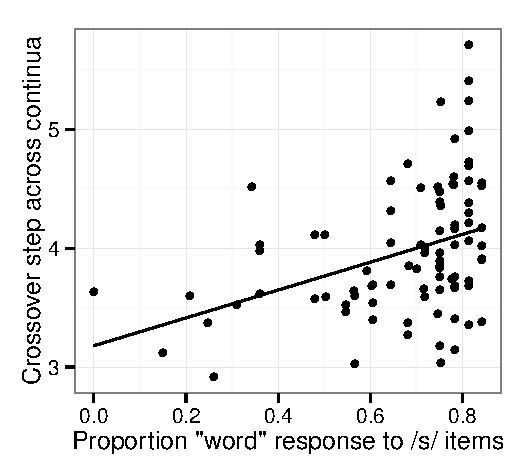
\includegraphics[width=80mm]{xoverwordresp}
\end{center}
\end{figure}

\section{Discussion and conclusion}



\bibliographystyle{icphs2015}
\bibliography{icphs2015}

\end{document}
